\documentclass[english]{article}

\usepackage{graphicx}
\usepackage{grffile}
\usepackage{babel}
\usepackage{float}

\textwidth = 426pt
\oddsidemargin = 17pt

\author{
	Jita, Hlengekile\\
	\texttt{14197520}
	\and
	Moodley, Joshua\\
	\texttt{150595538}
	\and
	Kazadi, Dieumerci\\
	\texttt{17308632}
	\and
	Nell, Stephan\\
	\texttt{15124861}
	\and
	Rayner, Peter\\
	\texttt{15312144}
	\and
	Van Hattum, Jason\\
	\texttt{15027458}
	\and
	Schuld, Bernhard\\
	\texttt{10297902}
}

\title{Architectural Requirements Specification\\
	for the NavUP System\\
	}
\date{\today}
\graphicspath{{Images/}}

\begin{document}
    \fboxsep=2mm

	\maketitle
	\begin{figure}[!t]
		
\includegraphics{up_logo.png}
	\end{figure}
	\pagenumbering{gobble}
	\newpage

	\tableofcontents
	\newpage

	\pagenumbering{arabic}


	\section{Introduction}
	
		This document will serve to outline the architectural requirements, constraints and design for the NavUP system. The general pattern that the system will be built around will also be discussed.\\
        \\
		In addition, the subsystems will be descried along with their planned implementation, accompanied by relevant diagrams. With regards to the subsystems, focus will be put onto designing the subsystems to be modular and loosely coupled in such a way that the system can be deployed with a minimal set of subsystems, and each subsystem can be changed without affecting the others.\\
		\\
		The modules that the document will outline are:
		\begin{itemize}
		    \item Data.
		    \item Users.
		    \item Navigation.
		    \item Surveillance.
		\end{itemize}

	\section{Overall System Design}
	    The system will be designed using the \textbf{n-tier} architecture (Specifically 3-tier), where the system is divided into three layers:
	    \begin{itemize}
	        \item Presentation Layer
	        \item Application Layer
	        \item Data layer
	    \end{itemize}

	    \subsection{Why}
	    This architecture brings several advantages:
	    \begin{enumerate}
	        \item Each layer will be modifiable without having to change the entire application.
	        \item As a result of the above, maintenance and adding extra functionality is easier.
	        \item Overall complexity of code over all layers will be reduced.
	        \item Layers are reusable in other applications.
	        \item As the system will likely be designed over several groups due to the nature of COS301, this will allow different groups to modify different layers without interference.
	        \item It is possible to deploy each layer (Specifically the data and application layers) over multiple different locations for better reliability and performance.
	    \end{enumerate}

	    \subsection{Presentation Layer}
	        This is the layer the user will be interacting with. It encompasses the actual apps (Android, iOS and web), and any interactions that the users have with them.

	    \subsection{Application Layer}
	        The application layer contains all the \textit{business logic} of the system - it makes logical decisions based on the interactions from the presentation layer and the data from the data layer.  \\
	        The decisions made by this layer include:
	        \begin{itemize}
	            \item Routes to be navigated.
	            \item Whether to allow a user to login/register.
	            \item Heatmap generation.
	            \item Creation and maintenace of a GIS Map of the Campus.
	            \item Treasure hunting activities by making use Geocaching.
	        \end{itemize}

	    \subsection{Data Layer}
	        The data layer is where the data and information used by the application layer is stored. This information includes:
	        \begin{itemize}
	            \item Student and staff information.
	            \item Waypoint history.
	            \item WiFi router locations.
	            \item Points of interest.
	            \item Information related to games and reward systems.
	            \item List of Events and their locations.

	        \end{itemize}

	   \subsection{Deployment}
	        \textless insert deployment diagram here\textgreater

	% ----- USERS ----- %
	\section{Users}
	    \begin{figure}[H]
            \centering	            \centerline{\fbox{\includegraphics[scale=0.4]{Class-Diagram-Users}}}
            \caption{Class Diagram - Users Module}
        \end{figure}

    % ----- NAVIGATION ----- %
	\section{Navigation}
        \subsection{Description}
            The purpose of the Navigation subsystem is to provide routes to users based on their destination and current location, as well as navigating the users along the route to their destination.\\
            This subsystem will reside almost entirely in the application layer, as it is comprised mostly of decisions related to navigation.

       \subsection{Requirements}
            The Navigation system should be able to:
            \begin{itemize}
                \item Provide a navigable route between two locations to a user on request, taking into account a possible set of preferences.
                \item Navigate a user from waypoint to waypoint until they arrive at their destination.
                \item Detect when a user deviates from their given route and recalculate a new route accordingly.
                \item Persist routes to the database for later use.
            \end{itemize}

        \subsection{Constraints}
            The system must operate under the following constraints:
            \begin{itemize}
                \item Any location data is received from the GIS subsystem, and is assumed to be correct.
                \item The destination is received from the user, and may be impossible to navigate to.
                \item The system has to work with the map as provided by GIS, which may have missing locations or locations that are incorrectly placed.
            \end{itemize}

        \subsection{Design}
            The Navigation system is implemented as 10 classes organised in two well-known design patterns - the Strategy and Memento patterns.

            \subparagraph{Strategy}
            The portion of the system which calculates routes is implemented in such a way that the algorithm can be changed easily by simple adding a class. This is done with the Strategy design pattern - each extra routing algorithm is simply added by adding a new class which inherits from \texttt{RouteAlgorithm}, and overrides the \texttt{calculate()} function. Decompiling each algorithm to a separate class will help with maintaining the code in the future and will reduce the overall complexity of the navigation module.

            \subparagraph{Memento}
            One of the requirements of the system is to save the route. The system will accomplish this by saving the waypoints as they are reached. The Memento design pattern is used here - each waypoint is saved as a \texttt{WaypointMemento} object to the database, which ensures that the state is unchanged when the object is recovered at a later stage.

        \begin{figure}[H]
            \centering	            \centerline{\fbox{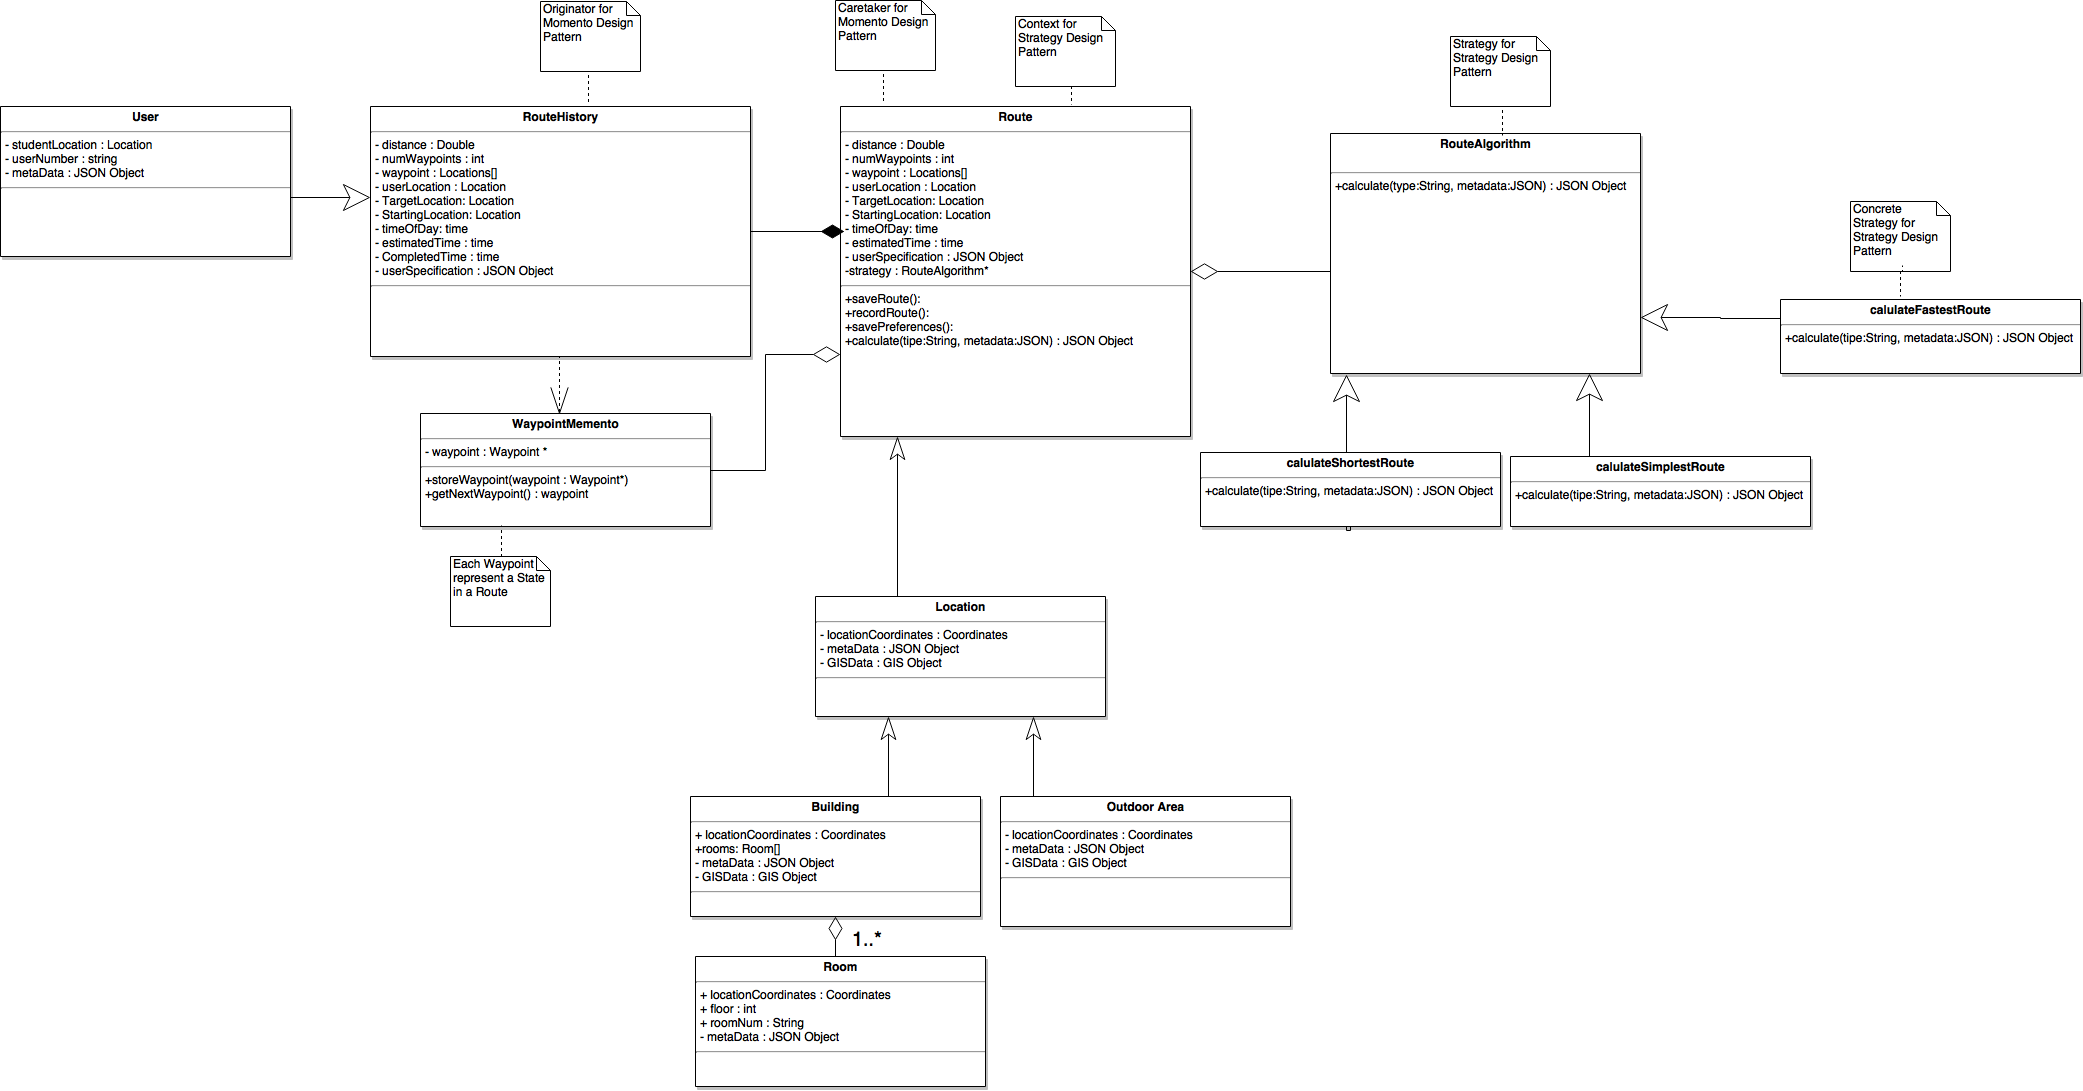
\includegraphics[scale=0.25]{Class-Diagram-Navigation.png}}}
            \caption{Class Diagram - Navigation Module}
        \end{figure}

        \subsection{Implementation Details}
            The system will, for the most part, be composed of a graph. In the graph each node would represent a location, with the links between the nodes representing the paths from location to location. \\
            Navigating from one location-node to another would then simply be a matter of using some shortest-path algorithm to find the path. The algorithm would depend on the user's preferences such as finding the shortest path as opposed to the quickest path, and so on. These algorithms would be interchangeable due to the use of the Strategy pattern. \\
            The nodes would be saved as \textit{Location} objects, and the route calculated by a \texttt{RouteAlgorithm} object.

        \begin{figure}[H]
            \centering	            \centerline{\fbox{\includegraphics[scale=0.75]{Graph-Navigation.png}}}
            \caption{Example Navigation Graph - Navigation Module}
        \end{figure}

        \begin{figure}[H]
            \centering	            \centerline{\fbox{\includegraphics[scale=0.45]{State-Diagram-Navigation.png}}}
            \caption{State Diagram - Navigation Module}
        \end{figure}

        \begin{figure}[H]
            \centering	            \centerline{\fbox{\includegraphics[scale=0.65]{Case-Diagram-Navigation.png}}}
            \caption{Use Case Diagram - Navigation Module}
        \end{figure}

    % ----- DATA ----- %
    \section{Data}
        \begin{figure}[H]
            \centering	            \centerline{\includegraphics[scale=0.5]{Data Use Case Diagram.png}}
            \caption{Use Case Diagram - Data Module}
        \end{figure}

        \begin{figure}[H]
            \centering	            \centerline{\fbox{\includegraphics[scale=0.5]{Data Activity Diagram.png}}}
            \caption{Activity Diagram - Data Module}
        \end{figure}

    % ----- SURVEILLANCE ----- %
    \section{Surveillance}
        \begin{figure}[H]
            \centering	            \centerline{\fbox{\includegraphics[scale=0.3]{Class-Diagram-Surveillance}}}
            \caption{Class Diagram - Surveillance Module}
        \end{figure}

        \begin{figure}[H]
            \centering	            \centerline{\fbox{\includegraphics[scale=0.5]{State-Diagram-Surveillance}}}
            \caption{State Diagram - Surveillance Module}
        \end{figure}

        \begin{figure}[H]
            \centering	            \centerline{\fbox{\includegraphics[scale=0.5]{Case-Diagram-Surveillance}}}
            \caption{Use Case Diagram - Surveillance Module}
        \end{figure}


\end{document}
>>>>>>> master
